%\chapter{Introduction}

\section{Motivation}

% More straightforward start?

With the steady rise in Earth's population and the consumption of natural resources, it has become essential to consider energy sustainability. The ever-increasing demand for energy accelerates, for example, the burning of fossil fuels, which not only contributes to the climate change but also rules out sustainability: the oil reserves are expected to run out in approximately 40 years with the present production rate \cite{}. Sustainable energy production therefore requires turning to more sustainable energy resources such as sun, wind, hydro- and, eventually, fusion power.

Sustainability cannot be reached, however, only by developing more efficient ways to produce energy: the efficiency of energy use should increase as well. At present, approximately half the energy produced in the world is wasted as heat \cite{}, and efficient reclaiming of even a small part of the waste heat using, e.g., thermoelectric modules could cover the electricity needs of the planet alone \cite{}. Inefficiency also hinders the technological development: in modern microprocessors, for example, the heating arising from energy dissipation is currently the most serious bottleneck limiting the performance \cite{}. 

Achieving more efficient thermoelectric modules and reducing the detrimental heating in electronic devices calls for engineering of new materials. Practically feasible thermoelectric generation requires, for example, materials with a low thermal conductivity but good electronic conduction properties \cite{chen}. Reducing the heating in electronic devices, on the other hand, can be achieved by reducing the thermal resistance of interfaces acting as heat bottlenecks and finding the optimal high thermal conductivity materials for heat sinks \cite{pop10}. 

Such thermal engineering has been largely enabled by the significant advancements in the field of nanophysics in recent decades. By allowing for the creation of new metamaterials with tailored thermal and electronic properties, nanostructuring has been shown to enable increasing the thermoelectric figures of merit in numerous materials (see, e.g., Refs. \cite{vineis10,kanatzidis10,shakouri11} for review). Similarly, interfacial resistance between dissimilar materials can be reduced by designing high thermal conductance interfaces by the addition of, e.g., functional molecules \cite{hopkins11,kaur14}, nanoscale thin films, and XXX between materials. Efficient extraction of heat from electronic and optoelectronic devices has been suggested \cite{ghosh08,yan12} to be enabled by low-dimensional nanomaterials such as graphene or carbon nanotubes, both having thermal conductivities higher than diamond \cite{balandin11}. 

The importance of nanostructures in thermal engineering is rooted in the break-down of classical heat transfer laws such as Fourier's law of thermal conduction \cite{fourier} or Planck's law of thermal radiation \cite{planck00a} in such small structures. Striking examples of break-down are, for example, the observation of thermal conductance quantization \cite{rego98,schwab00}, divergence of thermal conductivity in low-dimensional structures \cite{lepri97,lepri03,dhar08,xu14}, 100-fold reduction in nanowire's thermal conductivity compared to the bulk value \cite{hochbaum08} and the nearly monochromatic electromagnetic field close to a polar surface \cite{carminati99,shchegrov00}. In addition to the applications in thermoelectricity and electronics mentioned above, such novel heat transfer phenomena play an essential role also in completely new technologies such as phase-change memory \cite{lankhorst05}, heat-assisted magnetic recording \cite{pan09}, tumor therapy based on nanoparticle laser heating \cite{avedisian09}, and information processing using temperature \cite{li12_rmp}.  %In addition to leading to new understanding of physics, these phenomena offer new ways to engineer the thermal properties of materials.

Microscopically, energy transfer between materials is mediated by three primary energy carriers: photons, phonons, and electrons, which are responsible for electromagnetic, vibrational and electronic energy transfer, respectively \cite{chen}. While the contributions of different carriers to energy transfer between macroscopic bodies can typically be calculated independently from each other, this procedure breaks down as the separations between materials are in the nanometer range. For example, the correct description of the smooth transition from photon-dominated energy transfer at large separations to phonon-dominated transfer at small separations \cite{xiong14,chiloyan15} requires accounting both for electromagnetic fields and lattice vibrations in a single model. 


%Physically, such phenomena arise from the reduced dimensionality, wave interference effects, increased geometric scattering rates, reduced internal scattering and near-field effects appearing in nanoscale structures. 
%\begin{itemize}
 %\item Phase-change memory, heat-assisted magnetic recording
 %\item Thermal management of high-power electronic and optoelectronic devices
 %\item Thermoelectrics (Shiyun's citations \cite{hicks93}, \cite{Zhao2014})
 %\item Thermal therapy (intensely heated nanoparticles) \cite{jain08}
 %\item Biological applications (thermophoresis, DNA) \cite{jain11}
%\end{itemize}

%\begin{itemize}
% \item Half the world energy production is wasted as heat ($\sim 10^{13}$ TW), efficient reclaiming would cover the electricity demand
% \item Thermal rectifiers could act as energy harvesters
% \item Half the power consumed by data centers is spent on cooling, most limiting factor in performance
% \item Race to increase operating frequency stopped as local energy dissipation hit 100 W/cm$^2$, hotter than a hot plate
%\end{itemize}



\section{Scope and objectives}
% Smooth transition to scope and objectives, explain how different carriers play together at small scales
% Mapping of possibilities
% New computational methods
% Combining phononic, photonic and eventually electronic transport into a single model

This doctoral thesis aims at (i) developing new computational methods for investigating phononic energy transfer in nanoscale systems and applying the methods to create new understanding, and (ii) developing methods for describing phononic, photonic as well as electronic energy transfer in a single theoretical framework to eventually enable the combination of the models. In all our studies, we only consider solid state systems, thereby excluding convection from the considered list of energy transfer mechanisms. %We limit our scope to heat transfer by lattice vibrations and electromagnetic radiation, thereby excluding both electronic conduction and convection.

The two objectives listed above roughly divide the publications included in this thesis into two parts. In the first part, we use classical molecular dynamics (MD) simulations to model energy transfer by lattice vibrations (phonons) in nanoscale systems. While MD neglects all quantum effects, it accounts both for wave interference and detailed scattering phonon scattering without any approximations (except for typically using a semi-empirical potential for describing interatomic interactions). Using MD, we (1) study how interference and anharmonic scattering manifest in thermal transfer through a point contact, (2) investigate the detailed role of anharmonic scattering in energy transfer across a planar interface between two materials of different masses, and (3) develop a method for determining phonon scattering lengths from non-equilibrium MD (NEMD) simulations and use the method to determine scattering lengths in carbon nanotubes, and (4) demonstrate tunable thermal conductivity in twinning superlattice silicon nanowires.

In the second part, we pave the way for the unified theoretical description of phononic, photonic and electronic energy transfer. Our results show that Langevin theory \cite{langevin,zwanzig} combined with the linearization of equations of motion allows for calculating energy transfer rates for the three primary carriers in a unified manner. The solution of the Langevin equations of motion naturally gives rise to Green's functions, which act as response functions translating local stochastic fluctuations in carrier number into carrier propagation. Dissipative effects are mimicked by the coupling of the microscopic degrees of freedom such as atomic displacement or local dipole moment to the Langevin baths, giving rise to non-zero carrier relaxation times.

To put these research topics in the general context of nanoscale heat transfer, we briefly review the most prominent nanoscale energy transfer phenomena below and discuss their relation to each of the publications included in this thesis. 

%\begin{figure}
%\begin{center}
 %\includegraphics[width=8.6cm]{pics/schwab00_fig3.ps}
% 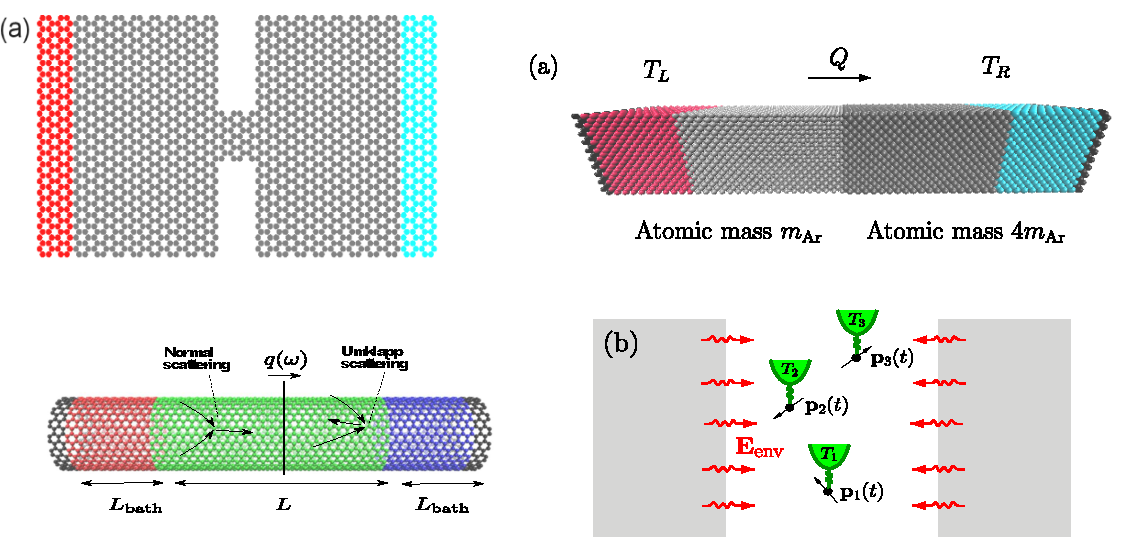
\includegraphics[width=.99\columnwidth]{pics/systems.pdf}
% \caption{Schematic illustration of some of the systems studied in this thesis. (a) Constriction in graphene. (b) Planar interface between two mass-mismatched face-centered cubic lattices. (c) Carbon nanotube. (d) Oscillating dipoles in a cavity.}
%\label{fig:intro_systems}
%\end{center}
%\end{figure}

%Some of the systems studied in this work are illustrated in Fig. \ref{fig:intro_systems}. First, we investigate interference effects and the effect of temperature on energy transfer and non-equilibrium temperature profiles in constrictions in two-dimensional lattices such as graphene, depicted in Fig. \ref{fig:intro_systems}(a). Interference effects are shown to give rise to intricately shaped temperature profiles in small constrictions, with increasing anharmonic scattering washing out the profiles. The work also clarifies the role played by the bulk reservoirs in heat transfer through low-dimensional systems. 

%We develop a computational method to determine the heat current carried by each vibrational frequency and apply the method to investigate the role of anharmonic phonon scattering on the thermal conductance of a planar interface depicted in Fig. \ref{fig:intro_systems}(b). The results show that anharmonic scattering can contribute to interfacial heat transfer both by presenting a dissipation mechanism for evanescent modes localized close to the interface and enabling three-phonon frequency-halving and frequency-doubling energy transfer processes at the interface. The same computational method is used to determine the phonon mean free paths in carbon nanotubes [Fig. \ref{fig:intro_systems}(c)] from non-equilibrium simulations, offering a novel method of determining the non-equilibrium scattering lengths in nanostructures and showing that mean free paths of energy carriers in carbon nanotubes can exceed 10 $\mu$m. In another work, we show that twinning Si nanowires could act as efficient thermoelectric materials due to their small thermal conductivity at a specific twinning period.

%Finally, we present a quantum Langevin equation-based approach on calculating electromagnetic energy transfer rates between oscillating dipoles and apply the theory to investigate the role of an inhomogeneous environment on electromagnetic energy transfer between nanoparticles. In addition to providing a new microscopic theory of electromagnetic energy transfer, we show that the confinement of electromagnetic modes in the mirror cavity [illustrated in Fig. \ref{fig:intro_systems}(d)] gives rise to oscillations in the heat transfer rates between polar nanoparticles as a function of particle distance. Heat transfer rate between nanoparticles is shown to be enhanced also close to a surface supporting surface phonon polaritons.



% Energy transfer between and inside bodies generally occurs by three mechanisms: conduction, radiation and convection \cite{}. 
%The energy transfer generally occurs by three mechanisms: conduction, radiation and convection \cite{}. Thermal conduction, which is the dominant mechanism in solids, is energy transfer inside a given body and occurs through (i) the microscopic interactions between the atoms and molecules constituting the body and, in case of metals, (ii) movement of free electrons. In fluids and gases, energy is transferred not only by conduction but also by the net motion of the energy-carrying molecules themselves, a process known as convection. As an example, the familiar law that hot air rises above the cold air is convection. Finally, energy can be transmitted by electromagnetic waves, i.e., thermal radiation. Unlike conduction and convection, thermal radiation does not require any mediating medium to carry energy: this is best exemplified by the thermal radiation from the Sun.

%The scope of this work is to investigate thermal conduction by lattice vibrations and electrons in nanoscale crystalline solids and thermal radiation between nanoparticles. In crystalline solids, lattice vibrations form propagating collective modes, the quanta of which are known as phonons. Below, we briefly review the main phenomena characteristic of thermal conduction in nanoscale. Detailed theory of lattice dynamics is presented in Chap. XXX.

% when the size of the structure or the scale of observations reaches nanoscale.

%\subsection{Experimental observations of }

%\begin{itemize}
% \item Interference, particles versus waves
% \item Boundaries and interfaces
% \item Ballistic versus diffusive, coherence
%\end{itemize}


\section{Energy transfer in nanoscale systems}
\begin{itemize}
 \item Phonon, photon, electron transport overlap
\end{itemize}
This Section reviews the prominent energy transfer phenomena of nanoscale systems. Vibrational energy transfer is reviewed in Subsection \ref{sec:intro_vib}. Emphasis is placed on the violations of the classical Fourier's law of heat transfer and defining the various length scales emerging in the microscopic scale. The mathematical theory underlying vibrational energy transfer is presented in detail in Chap. \ref{chap:theory}. 

% Because this thesis mainly focuses on phonon and photon transport, more emphasis is placed on these transfer mechanisms. 

Electromagnetic energy transfer phenomena in nanoscale are reviewed in Subsection \ref{sec:intro_em}. In electromagnetic energy transfer, the macroscopic laws of thermal radiation such as Planck's radiation law break down when the separation between bodies becomes similar to the wavelengths of thermally excited electromagnetic fields. At such small separations, evanescent near-fields localized close to the material surfaces can couple the materials and thereby strongly increase energy transfer rates. %The near-field energy transfer is reviewed in Subsection \ref{sec:intro_em}.

Subsection \ref{sec:intro_electrons} reviews electronic conduction of heat in metallic and semi-conducting nanostructures. Because electron transport topics such as electron conductance quantization, Coulomb blockade, localization etc. are outside the scope of this thesis, Subsection \ref{sec:intro_electrons} is only devoted to the discussion of electronic heating in nanostructures. %These effects include the generation of hot spots and the possibility to measure thermal conductivity from local heating. %detrimental electronic heating has been suggested to be reduced by low-dimensional, high thermal conductivity materials

% Hot spots
% Graphene quilts etc.
% Measurement of thermal conductivity from Joule heating 
% Conductance at metal-dielectric interfaces
% Current induced forces?

% Similarity of phonon, photon systems (interference, scattering, Green's function methods,...)

\subsection{Vibrational energy transfer in nanoscale}
\label{sec:intro_vib}
% Start from Peierls's theory
The microscopic theory for thermal conduction was developed by Rudolf Peierls in 1929 \cite{peierls29}. Understanding that collective lattice vibrations (phonons) carry heat in crystalline solids, he proposed that thermal resistivity arises from the scattering of phonons from lattice imperfections and other phonons. These scattering mechanisms existing in any non-ideal material at non-zero temperature give rise to a finite phonon mean free path, characterizing the average distance between scattering events. At length scales much larger than the mean free path, the heat carriers are expected to essentially perform a random walk with constant drift along the temperature gradient and heat transfer is well described by Fourier's local theory. At length scales smaller than the mean free path, on the other hand, phonons can travel without scattering and Fourier's theory must be invalid. 

% Thermal conduction in macroscopic systems is traditionally described using Fourier's law \cite{fourier}, stating that the heat flux at any given point is proportional to the temperature gradient at the same point. The theory leads, however, to the unphysical phenomenon that a local temperature perturbation can propagate infinitely fast \cite{chen}, in direct contradiction to the finiteness of the speed of sound and also special relativity. This indicates that Fourier's theory must ultimately break down in nanoscale.

This expected transition to the Fourier limit in sufficiently large systems has been questioned in recent decades by computer simulations \cite{lepri97,lepri03,mai07,dhar08} and heat transfer experiments \cite{yang10,xu14} indicating that the Fourier limit may never be reached in low-dimensional systems. In one-dimensional oscillator chains, for example, it is now widely accepted \cite{dhar08} that the thermal conductivity diverges as a function of system length following a power-law \cite{mai07}. It is, however, still debated \cite{marconnet13} if any physical system such as a nanowire can be treated as a one-dimensional object and could therefore exhibit the divergence. %Some experiments have claimed to have observed such anomalous thermal conduction in silicon nanowires \cite{yang10}, but the evidence remains inconclusive. % In two-dimensional materials such as graphene, similar divergence is expected, and recent experiments and simulations for graphene have suggested this to be the case \cite{xu14}. %\citepub{cnt}

\begin{figure}
\begin{center}
 %\includegraphics[width=8.6cm]{pics/schwab00_fig3.ps}
 \includegraphics[width=8.6cm]{pics/schwab00_fig3.pdf}
 \caption{Thermal conductance measured as a function of temperature by Schwab \textit{et al.} \cite{schwab00}. In their experimental setup, heat was transferred through four nanowires with four acoustic modes in each carrying the heat. The measured conductance at low temperature is therefore $G=16g_0$, where $g_0$ is the conductance quantum. Reprinted with permission from Ref. \cite{schwab00}.}
\label{fig:intro_schwab}
\end{center}
\end{figure}

In systems smaller than the phonon mean free path, on the other hand, Fourier's law is undisputably invalid due to the scattering-free propagation of heat carriers. Such bullet-like transport of phonons is called ballistic transport, contrasting with the diffusive transport of Fourier-like systems. The most striking example of ballistic transport is the thermal conductance quantization, predicted theoretically by Rego and Kirczenow in 1998 \cite{rego98}. Their calculations showed that at sufficiently low temperatures, where phonon scattering is minimal and only the lowest-frequency phonon modes can be excited, thermal conductance through a narrow constriction is an integer multiple of the thermal conductance quantum. The thermal conductance quantum, which is analogous to the quantum of electrical conductance, is independent of any material properties and only depends on temperature and Planck's constant. The predicted quantization was observed experimentally in 2000 by Schwab \textit{et al.} \cite{schwab00} (see Fig. \ref{fig:intro_schwab}), thereby indirectly confirming also the existence of ballistic transport.

In addition to the mean free path, there is another internal length scale governing heat transfer, the phonon wavelength. In devices smaller than or of the same size as dominant phonon wavelength, interference effects appear. Interference effects have enabled designing acoustic reflectors with novel applications in enhancing the optical-mechanical coupling \cite{fainstein13} and phonon lasing \cite{maryam13}. Wavelength-related effects are also useful in thermal engineering: as an example, Kim \textit{et al.} were able to reduce the thermal conductivity of InGaAs alloy (which naturally scatters short-wavelength phonons due to point defects) by introducing nanoparticles acting as scatterers for mid-to-long-wavelength phonons \cite{kim06}. %\citepub{fpu}\citepub{fpu2}\citepub{gf} % Other examples of interference

In a nanoscale system with relatively long internal phonon mean free paths, the material surfaces and interfaces play an important role in thermal conduction. At rough surfaces, for example, phonons are scattered into all directions, which strongly suppresses the heat flow. The resulting reduced thermal conductivity has been noted to be responsible for the moderately high thermoelectric figure of merit of Si nanowires \cite{hochbaum08}. At material interfaces, the mismatch in the acoustic properties of the materials inevitably scatters phonons.  This contact resistance between dissimilar materials can act as a major bottleneck limiting the extraction of heat from electronic devices, thereby hindering their performance \cite{pop10}. Many methods have been suggested to reduce the thermal resistance between materials, including chemical functionalization \cite{hopkins11,kaur14}, external pressure \cite{shen11,chalopin12}, and heat-mediating thin films \cite{english12}. %\citepub{spectral}\citepub{twinning}

% Relation to the thesis
Concepts such as phonon interference, ballistic transport, mean free paths, and interface scattering appear throughout this thesis. In Publications \cp{fpu}, \cp{fpu2}, and \cp{gf}, we explore the interference effects exhibited in thermal conduction through nanoscale constrictions and reveal intricate interference patterns in local nonequilibrium temperature profiles. We also show how such patterns vanish at higher temperatures due to increased scattering. In Publication \cp{spectral}, we present detailed maps of the contributions of different vibrational frequencies to thermal conduction across a mass-mismatched interface, improving thereby the understanding of heat transfer mechanisms at interfaces and presenting guidelines for future thermal engineering of high-conductance interfaces. Publication \cp{cnt} presents a non-equilibrium method for determining the mean free paths of phonons in carbon nanotubes, supplying a theoretical description of the ballistic-diffusive crossover in one-dimensional systems. In Publication \cp{twinning}, we perform ''thermal engineering'' and demonstrate the existence of minimun thermal conductivity at a certain twinning period length in a silicon nanowire. The minimun arises from the maximal blocking of bulk-like scattering-free propagation of phonons through the nanowire by the periodically repeating twinning boundaries.


%As noted by Kapitza already in 1930s \cite{}, carrier scattering at interfaces between materials also gives rise to thermal resistance. Even in the absence of defects, 

% Point contacts \cite{bartsch12}

% Contact resistance is a bottleneck
% Material properties increasingly dominated by interfaces

% Interfaces

% Superlattices, phonon mirrors

% While there is convincing evidence from numerical simulations that the Fourier limit is always achieved in three-dimensional systems \cite{saito10,wang10}, this seems not to be the case in one- or two-dimensional systems. Numerical simulations \cite{lepri97,mai07} and hydrodynamical theory \cite{} suggest that the thermal conductivity in one-dimensional systems diverges in a power-law fashion as a function of system length, but clear experimental demonstration of the divergence has not been achieved so far. In two-dimensional systems, thermal conductivity is expected to diverge logarithmically \cite{}. Recent experiments claim to have observed the divergence in graphene \cite{xu14}.

%\subsection{Thermal boundary resistance}

%\subsection{Thermal engineering}

\subsection{Electromagnetic energy transfer in the near-field}
\label{sec:intro_em}
Accelerating charges are known to emit electromagnetic radiation \cite{}. Because the electrons and nuclei in any solid material undergo thermal (and quantum) fluctuations, all materials therefore emit electromagnetic radiation carrying heat. In 1900, Max Planck \cite{planck00a} studied the radiation emitted by a blackbody and gave birth not only to quantum theory but also to Planck's blackbody radiation law, which has since been observed to describe, for example, the spectrum of cosmic microwave background radiation at the accuracy of XXX.

Planck's law inherently suggests that the total power of the emitted radiation is independent of the distance from the object. This follows from the assumption that only propagating waves contribute to the energy density. Close to the material surface, solution of Maxwell's equations gives, however, also rise to evanescent electromagnetic fields localized at a distance of a few wavelengths from the object \cite{polder71}. One can then envisage placing another object sufficiently close to the radiating body so that the evanescent fields can induce motion of charges in the added object, leading to energy transfer by the evanescent fields. Planck's law therefore breaks down at very small distances. 

The breakdown in Planck's law was first observed by Hargreaves \cite{hargreaves69}, who found an enhancement in the heat transfer rate between two chromium layers as the layers were separated by subwavelength gap. The theoretical calculation for the exact enhancement rate was carried out by Polder and van Hove \cite{polder71}, and consequently near-field enhancement effects were predicted in numerous geometries \cite{loomis94,pendry99,carminati99,shchegrov00,mulet01,volokitin01}. In the last decade, advances in experimental techniques have allowed for very precise measurements of near-field enhancement rates \cite{}, confirming the experimental predictions. Near-field effects are now routinely used in thermal microscopy \cite{majumdar99,muller-hirsch99,kittel05,kittel08}. They are also expected to give rise to engineering applications in, e.g., infrared thermophotovoltaics \cite{dimatteo01,narayanaswamy03,laroche06} and building narrow-band infrared antennas \cite{greffet02}. 

\begin{figure}
\begin{center}
 %\includegraphics[width=8.6cm]{pics/schwab00_fig3.ps}
 \includegraphics[width=8.6cm]{pics/shchegrov00_fig1.pdf}
 \caption{The spectral energy density of electromagnetic field (arbitrary units) close to a SiC surface at distances of (a) $1$ mm, (b) $2$ $\mu$m, and (c) $100$ nm. At the distance of 100 nm, the spectral energy density is dominated by the surface phonon polariton at frequency $\omega=178.7$ Trad/s, resulting in essentially monochromatic energy emission. Inset show the spectral energy densities plotted in semilogarithmic scale. Reprinted with permission from Ref. \cite{shchegrov00}.}
\label{fig:intro_shchegrov}
\end{center}
\end{figure} 

Near-field effects are particularly strong for materials supporting evanescent surface waves decaying at both sides of the surface \cite{shchegrov00}. The surface waves arise from the coupling between the electromagnetic field and either the free electrons (surface plasmon polaritons) or transverse optical phonons (surface phonon polaritons). While surface plasmon polaritons can only be thermally excited in metals at temperatures much higher than room temperature, surface phonon polaritons can contribute to thermal transfer in polar semiconductors even at room temperature. To demonstrate the large contribution of surface waves, Fig. \ref{fig:intro_shchegrov} shows the theoretically calculated \cite{shchegrov00} spectral energy density of the electromagnetic field at various distances from a SiC surface.

Similarly, near-field effects strongly increase the spectral density of the electromagnetic field in the vicinity of nanoparticles made of a polar material. Consequently, heat transfer between two nanoparticles in vacuum is found to strongly increase at small distances \cite{domingues05}. In practice, however, the required nanoparticle distances for efficient heat transfer may be too small, so for practical applications it would be necessary to engineer the thermal conductance to be higher. From the theory of dipole emission, it is well known that the optical-mechanical coupling can be enhanced by orders of magnitude in an inhomogeneous environment such as in a mirror cavity \cite{novotny}. This raises the question, if the interparticle heat transfer rate between particles could be enhanced by cavity. This question was investigated and answered in positive in \citepub{dipole}.


\subsection{Thermoelectricity and Joule heating in nanostructures}

 %it has a few problems. First, multiple different microscopic definitions for the polarizability exist, varying on whether the polarizability expresses the response, e.g., to the total electric field consisting of the external field and the internal polarization field or only the external field. This ambiguity is related to the observation of Manjavacas and Garc\'ia de Abajo \cite{manjavacas12} that Eq. \eqref{eq:th_fed_fdt} can be used to predict unphysical fluctuations even in a non-absorbing medium. The imaginary part of polarizability must, after all, be strictly positive even in a non-absorbing medium due to the radiation reaction force, but a non-absorbing medium cannot emit radiation.  % Even in a non-absorbing medium, the imaginary part of the polarizability is non-zero due to the radiation reaction force. Therefore, Eq. \eqref{eq:th_fed_fdt} predicts unphysical fluctuations even in absence of actual dissipation.

%A second difficulty in Eq. \eqref{eq:th_fed_fdt} is that it does not simply allow for coupling of, say, acoustic and optical degrees of freedom. 



%Electromagnetic energy transfer between dielectric bodies at different temperatures is commonly described using the fluctuational electrodynamics theory developed by Rytov. The theory describes the radiation generated by thermal motion of charges and its connection to the dissipation captured by the imaginary part of the polarizability. 


%Following theoretical developments and advances in experimental techniques, near-field 
%The theory has since been used to theoretically predict strong near-field enhancements of heat transfer in various geometries \cite{loomis94,pendry99,mulet01,volokitin01}. 

% Surface polaritons

% The theoretical calculation of the exact near-field enhancement was consequently carried out by Polder and van Hove \cite{polder71}, who applied the fluctuational electrodynamics theory developed by Rytov \cite{rytov58}. 



%The predictions have been explored in more detail also experimentally [13-18]. 
\iffalse
Electromagnetic energy transfer between dielectric bodies at different temperatures is commonly described using the fluctuational electrodynamics (FED) approach \cite{joulain05,volokitin07} developed by Rytov \cite{rytov58,rytov} and first applied to condensed matter physics by Lifshitz \cite{lifshitz55,lifshitz56}. According to FED, thermal motion of charged particles in a body creates random currents, which induce electromagnetic fields. Outside the body, the field is then either radiated to free space or absorbed in the near or far-field regime by another body. In the near-field, the heat transfer rate between bodies can surpass the Planckian blackbody limit \cite{planck} by several orders of magnitude, as first suggested theoretically \cite{polder71,pendry99,carminati99,shchegrov00,mulet01,volokitin01} and later confirmed experimentally \cite{kittel05,hu08,rousseau09,shen09,ottens11}. Near-field enhancement of heat transfer is expected to have numerous applications in, e.g., thermal microscopy \cite{majumdar99,muller-hirsch99,kittel05,kittel08}, infrared thermophotovoltaics \cite{dimatteo01,narayanaswamy03,laroche06} and narrow-band infrared antennas \cite{greffet02}.
\fi


%As early as 1884, John Poynting calculated the energy flux carried by propagating electromagnetic waves. 


\iffalse
\section{Summary of experimental techniques}

\subsection{Thermal conductivity}

\begin{itemize}
 \item $3\omega$ technique
 \item Picosecond ultrasonic techniques (transient reflectance)
\end{itemize}

\subsection{Local temperature}

\subsection{Electromagnetic near-field transfer}

\subsection{Scanning thermal microscopy}

Measure the temperature of an AFM probe during the scan using either a thermocouple junction (measure voltage caused by temperature change) or microbolometer technique (measure change in resistance). In the latter, two leads are connected at the end of the probe by a Joule heating element which can be used either for temperature measurement by measuring its temperature change or for heating by driving current through it. In the constant power mode, the resistance of the heating element is measured by measuring the voltage in a Wheatstone bridge. If the voltage is fed back to the contact voltage, one can keep constant temperature at the resistor. 

Heat flow from the tip can be due to
\begin{itemize}
 \item Solid-solid conduction (this is what is wanted)
 \item Liquid-liquid conduction by the liquid meniscus between the tip and the sample, use UHV conditions
 \item Gas-gas conduction, use UHV conditions
 \item Near-field radiation between the tip and the sample
 \item Heat flow to cantilever
\end{itemize}

If the temperature of the tip, say, drops during the scan, this can be due to (a) lower local temperature, or (b) higher thermal conductivity at the sample spot. Also lower heat capacity is possible (?). 

Technique developed by Nonnenmacher (1992), Wickramasinghe (1992), Majumdar (1993), Pilkki (1994), etc.

Other methods to measure temperature are (see the review by Yue and Wang)
\begin{itemize}
 \item Optical methods based on the temperature-dependence of Raman or fluorescence signal of the measuring target (molecule, nanoparticle, etc.), which can also be used as the temperature sensor at the tip of an AFM, for example
 \item Near-field optical temperature measurement, with or without aperture
\end{itemize}

\subsection{Inelastic neutron scattering}
 \begin{itemize}
  \item Neutrons interact strongly only with the atomic nuclei (dipole scattering etc. typically weaker)
  \item Map the change in the neutron energy and momentum, one-phonon scattering processes sharply resolved among the multi-phonon process background
  \item Vary neutron energy, orientation of crystal and detection direction
  \item Gives phonon dispersion relations and broadenings, anharmonic effects mapped recently e.g. in doi:10.1038/nmat3035 and doi:10.1038/nnano.2013.95
 \end{itemize}
\fi
